\chapter{페ン로즈 다이어그램과 실제 블랙홀의 형성}

크루스칼 그림은 슈바르츠실트 지평선 주변을 우아하게 묘사하지만, 실제 블랙홀은 영원히 존재하는 것이 아니다. 물질이 붕괴할 때 형성된다. 확장된 그림 가운데 이러한 물리적 역사를 거친 뒤에도 남는 부분은 무엇일까? 이 질문에 답하려면 시공간 전체를 담을 만큼 크면서 빛의 운동을 제대로 보존하는 다이어그램이 필요하다. 먼저 평탄 시공간을 콤팩트화하고, 이어서 슈바르츠실트 시공간을 콤팩트화한 다음, 유입하는 복사 껍질을 경계로 적절한 부분들을 이어 붙이겠다.

\section{지평선 근처: 크루스칼 그림 복습과 네 사분면}

앞선 강의가 끝난 바로 그 지점에서 시작하자. 슈바르츠실트 지평선 바로 근처의 기하학은 국소적으로 평탄한 공간처럼 보인다. 지평선 자체는 쌍곡선 극좌표의 자취처럼 거동하는데, 이는 보통의 민코프스키 시공간에서 가속 좌표가 보이는 양상과 비슷하다. 이 국소적인 그림에서는 처음부터 한 가지 규칙을 정하고 끝까지 지킨다. 반지름 방향 빛줄기는 \(45^\circ\)로 그리며, 모든 시간꼴 세계선은 그 영선들보다 더 가파르게 놓여야 한다.

이 복습에서 쓰는 좌표는 자유 낙하 관찰자가 보는 시간과 공간으로 생각하는 것이 가장 좋다. 이 국소 관성 좌표에서 지평선 주변은 거의 평탄해 보인다. 그러나 블랙홀 바깥에서 반지름을 고정한 채 정지해 있으려는 관찰자는 관성계에 있지 않다. 자유 낙하계에 비해 그런 관찰자는 가속 곡선을 그린다. 지평선에 가까이 정지해 있을수록 벗어나지 않기 위해 필요한 가속도는 커진다. 이것이 칠판 오른쪽에 그려진 바깥쪽 곡선들의 물리적 의미다.

\begin{figure}[htbp]
\centering
\includegraphics[width=0.72\textwidth]{lecture_08_figure_02.png}
\caption{지평선 근처 네 영역 기하학을 칠판에 그린 스케치. 바깥쪽의 빨간 곡선은 반지름을 고정한 채 정지해 있는 세계선들의 한 계열을 나타낸다.}
\lectureframe{00:02:54}
\end{figure}

\begin{figure}[htbp]
\centering
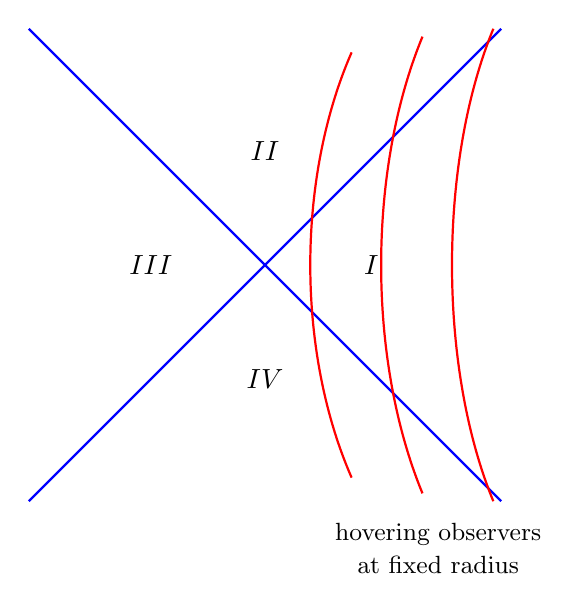
\begin{tikzpicture}[scale=1.0]
\draw[thick,blue] (-3,3) -- (3,-3);
\draw[thick,blue] (-3,-3) -- (3,3);

\draw[red,thick] (1.1,-2.7) .. controls (0.4,-1.1) and (0.4,1.1) .. (1.1,2.7);
\draw[red,thick] (2.0,-2.9) .. controls (1.3,-1.2) and (1.3,1.2) .. (2.0,2.9);
\draw[red,thick] (2.9,-3.0) .. controls (2.2,-1.3) and (2.2,1.3) .. (2.9,3.0);

\node at (1.35,0.0) {$I$};
\node at (0.0,1.45) {$II$};
\node at (-1.45,0.0) {$III$};
\node at (0.0,-1.45) {$IV$};

\node[align=center] at (2.2,-3.6) {\small hovering observers\\\small at fixed radius};
\end{tikzpicture}
\caption{복습에서 사용한 크루스칼식 인과 구조를 깔끔하게 다시 그린 그림. 영역 \(I\)는 바깥 영역이고, 영역 \(II\)는 빠져나올 수 없는 내부 영역이다. 영역 \(III\)과 \(IV\)은 형식적 확장에 속하며, 실제로 붕괴해 형성된 블랙홀에서는 나중에 버릴 부분이다.}
\end{figure}

이 그림만으로도 블랙홀이 어떤 일을 하는지 말할 수 있다. 바깥 영역 \(I\)에서는 물체와 신호가 안쪽으로 갈 수 있지만, 바깥에 머물거나 다시 밖으로 돌아설 수도 있다. 반면 영역 \(II\)에서는 인과적 결론이 정해져 있다. 일단 내부에 들어가면 미래 방향의 인과 경로를 따라 바깥 영역으로 돌아올 수 없다. 영역 \(II\)에서 바깥쪽 두 영역 가운데 어느 곳으로든 빠져나가려면 어딘가에서 \(45^\circ\)보다 완만한 궤적을 따라야 하므로 빛보다 빨라야 한다. 허용되는 모든 미래 방향 시간꼴 궤적은 특이점에서 끝난다.

이 도입부의 복습은 단순한 반복이 아니다. 이 장의 핵심 주제를 준비한다. 크루스칼 그림은 유용하지만, 실제 블랙홀에 물리적 의미가 있는 것은 그 전부가 아니다.

\begin{classroomqa}
\audiencequestion{다이어그램의 축은 무엇이며, 빨간 곡선은 어떤 관찰자들의
고정 위치 세계선인가요?}
\lecturerresponse{축은 자유 낙하 관찰자에게 자연스러운 좌표에서의 시간과
공간입니다. 지평선 근처에서 이 관찰자는 거의 평범한 평탄 시공간을 봅니다.
반면 빨간색 위치 고정 곡선은 블랙홀 바깥에 정지해 있도록 붙들린 관찰자들의
세계선입니다. 이들은 가속 운동을 하며, 지평선에 가까울수록 필요한 가속도가
커집니다.
\lecturetimestamp{00:05:58--00:06:47}}
\end{classroomqa}

\section{왜 콤팩트화하는가? 무한한 시공간에서 유한한 칠판으로}

다음 단계는 방법론적인 것이다. 이 다이어그램에서 영 방향들은 무한대로 뻗고 시간 자체도 무한히 흐른다. 따라서 좌표를 바꾸지 않고는 보통 칠판에 시공간 전체를 그릴 수 없다. 강의자의 동기는 아주 구체적이다. 모든 것을 한눈에 보고 전역적인 인과 구조를 따져 보려면, 빛줄기를 알아볼 수 있게 유지하면서 무한한 시공간을 유한한 영역으로 압축할 방법이 필요하다.

그래서 먼저 쉬운 경우, 익숙한 평탄 시공간으로 돌아간다. 관심 있는 문제가 구대칭이므로 각도 방향은 생략하고 시간과 반지름 좌표만 남긴다. 좌표 \(T\)와 \(R\)를 사용하며,
\[
R\ge 0,
\]
극좌표에서 음의 반지름은 의미가 없기 때문이다. 또한 다음과 같은 단위계를 택한다.
\[
c=1.
\]
이 약속에 따르면 반지름 방향의 영운동은 \(45^\circ\)로 그려진다.

콤팩트화 사상을 도입하기 전에, 강의에서는 \(T\)-\(R\) 평면에서 방향을 잡는 데 시간을 들인다. 시간축과 반지름축, 몇 개의 시간 고정 단면 \(T=0,\pm1,\pm2\), 그리고 몇 개의 반지름 고정 선 \(R=1,2,3\)을 그린다. 이것은 무의미한 형식 절차가 아니다. 기준점을 제공하고, 나중에 다이어그램을 유한한 크기로 압축할 때 어떤 특징을 보존하려는지 분명히 해 준다.

원점에 관한 미묘하지만 중요한 교육적 요점도 있다. 축약된 반지름 그림에서는 정확히 \(R=0\)를 향한 빛줄기가 원점에서 튕겨 나와 되돌아가는 것처럼 보인다. 그러나 물리적으로 어떤 벽에서 반사되는 것은 아니다. 완전한 구대칭 기하학에서는 빛줄기가 원점을 통과해 반대편으로 나온다. 겉보기의 반사는 반평면 \(R\ge 0\)에서 작업한 결과일 뿐이다.

마찬가지로 원점을 비껴가는 빛줄기도 처음에는 거의 같은 모습으로 출발해 최근접점에 이른 뒤 바깥쪽으로 되돌아간다. 이 좌표에서는 무언가가 빛줄기를 원점에서 밀어낸 것처럼 보일 수도 있다. 그러나 이것 역시 새로운 힘이 아니라 익숙한 각운동량 장벽을 좌표로 표현한 것이다. 강의자가 이런 사례들을 오래 설명하는 것은 다이어그램을 변형하기 전에 청중이 이를 신뢰하게 하려는 것이다.

이제 핵심 단계에 이르렀다. 그림을 압축하고 늘리되 한 가지는 그대로 유지한다. 반지름 방향 빛줄기는 계속 \(45^\circ\) 선으로 그려야 한다. 이것이 콤팩트화의 핵심이다.

\begin{classroomqa}
\audiencequestion{선택한 원점에는 물리적으로 특별한 점이 있나요? 겉보기에
휘어진 빛줄기는 그곳에 힘이 작용한다는 증거인가요?}
\lecturerresponse{아닙니다. 이 단계에서 원점은 구면좌표가 선택한 중심일 뿐입니다.
겉보기의 반사와 휘어짐은 완전한 공간 운동을 \(R\geq0\)로 축약한 데서
나타납니다. 태양의 경우처럼 대칭성 때문에 중심이 편리할 수는 있지만,
좌표를 그렇게 정했다고 해서 그곳에 블랙홀이나 반사벽이 생기는 것은 아닙니다.
\lecturetimestamp{00:16:27--00:17:08}}
\end{classroomqa}

\section{영좌표와 페ン로즈 형식으로 나타낸 평탄 시공간}

변형을 정확히 다루기 위해 영좌표를 도입한다. 이것은 강의의 수학적으로 깔끔한 부분이며, 칠판에서 그 단계가 명시적으로 드러난다.

\begin{figure}[htbp]
\centering
\includegraphics[width=0.82\textwidth]{lecture_08_figure_03.png}
\caption{도입부에서 비워 둔 \(T\)-\(R\) 칠판. 축약된 반지름 좌표의 원점은 파란색 수직선 \(R=0\)이다. \(T^+=T+R\)와 \(T^-=T-R\)도 표시되어 있다.}
\lectureframe{00:19:45}
\end{figure}

다음과 같이 정의한다.
\begin{align}
T^+ &= T+R, \\
T^- &= T-R.
\end{align}
이 좌표들은 반지름 방향 영운동에 맞춰져 있다. 안쪽으로 향하는 반지름 방향 빛줄기에서는 \(T^+=\text{const}\)이고, 바깥쪽으로 향하는 빛줄기에서는 \(T^-=\text{const}\)이다.

\paragraph{계산 유도.}
이 좌표에서는 선 \(R=0\)가 특히 간단한 형태를 띤다. 실제로,
\begin{align}
R=0
&\iff T+R=T-R \\
&\iff T^+=T^-.
\end{align}
따라서 시간꼴 경계 전체 \(R=0\)는 다음 하나의 관계로 표현된다.
\begin{equation}
R=0 \iff T^+=T^-.
\end{equation}

\begin{figure}[htbp]
\centering
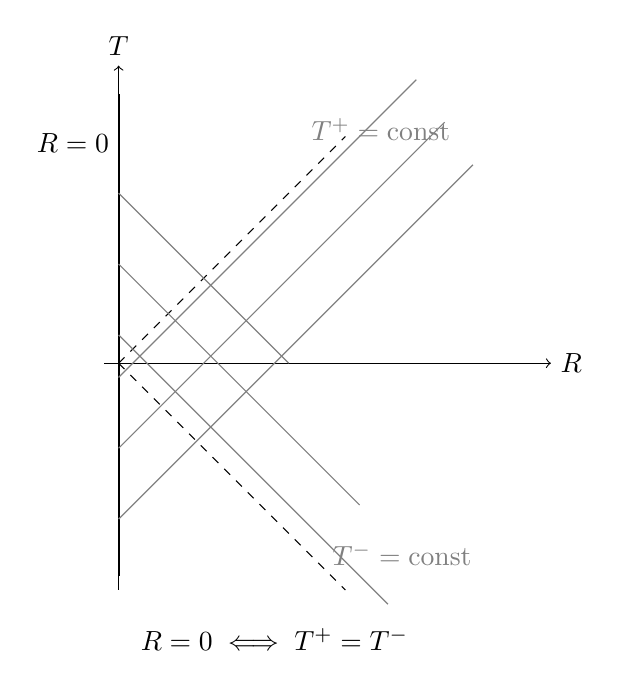
\begin{tikzpicture}[scale=0.9]
\draw[->] (-0.2,0) -- (6.1,0) node[right] {$R$};
\draw[->] (0,-3.2) -- (0,4.2) node[above] {$T$};

\draw[thick] (0,-3.0) -- (0,3.8);
\node[left] at (0,3.1) {$R=0$};

\draw[dashed] (0,0) -- (3.2,3.2);
\draw[dashed] (0,0) -- (3.2,-3.2);

\draw[gray] (0,2.4) -- (2.4,0);
\draw[gray] (0,1.4) -- (3.4,-2.0);
\draw[gray] (0,0.4) -- (3.8,-3.4);

\draw[gray] (0,-2.2) -- (5.0,2.8);
\draw[gray] (0,-1.2) -- (4.6,3.4);
\draw[gray] (0,-0.2) -- (4.2,4.0);

\node[gray] at (3.7,3.3) {$T^+=\mathrm{const}$};
\node[gray] at (4.0,-2.7) {$T^-=\mathrm{const}$};

\node at (2.2,-3.9) {$R=0 \iff T^+=T^-$};
\end{tikzpicture}
\caption{깔끔하게 다시 그린 \(T\)-\(R\) 그림. 두 영 방향 계열은 \(T^+\)와 \(T^-\)의 등위선이며, 선 \(R=0\)은 같은 뜻으로 \(T^+=T^-\)이라고 쓸 수 있다.}
\end{figure}

이제 콤팩트화한다. 새로운 영좌표 \(U^\pm\) 두 개를 도입한다. 각각은 대응하는 \(T^\pm\)에 같은 유계 단조함수 \(F\)를 적용해 얻는다.
\begin{align}
U^+ &= F(T^+), &
U^- &= F(T^-),
\end{align}
여기서
\begin{equation}
F(+\infty)=1,
\qquad
F(-\infty)=-1.
\end{equation}
강의에서 편리하게 택한 함수는 다음과 같다.
\begin{equation}
F(x)=\tanh x,
\end{equation}
따라서
\begin{equation}
U^+ = \tanh(T^+),
\qquad
U^- = \tanh(T^-).
\end{equation}
쌍곡탄젠트 함수 자체에 특별한 의미가 있는 것은 아니다. 적절한 극한 거동을 갖는 매끄러운 함수일 뿐이며, 그 덕분에 무한한 좌표 범위를 유한한 범위로 압축할 수 있다.

영 구조가 보존되는 이유는 간단하다. 안쪽으로 향하는 반지름 방향 빛줄기에서 \(T^+=\text{const}\)라면,
\[
U^+=F(T^+)=\text{const},
\]
마찬가지로 바깥쪽으로 향하는 반지름 방향 빛줄기에서 \(T^-=\text{const}\)라면,
\[
U^-=F(T^-)=\text{const}.
\]
따라서 콤팩트화는 두 영 방향을 각각 재매개화하며, 반지름 방향 빛줄기는 계속 \(45^\circ\) 선으로 남는다. 원점 선도 다음과 같이 그대로 옮겨진다.
\[
T^+=T^- \Longrightarrow U^+=U^-.
\]

이제 평탄 시공간의 무한한 반평면이 유한한 삼각형으로 압축되었다. 이어서 강의에서는 그 가장자리들을 읽는 법을 알려 준다. 공간 무한대는 하나의 점 \(i^0\)으로 수축된다. 미래와 과거의 시간꼴 무한대는 각각 \(i^+\)와 \(i^-\)이다. 두 영 가장자리는 각각 \(\mathcal{I}^+\)와 \(\mathcal{I}^-\)이며, 흔히 스크라이 플러스와 스크라이 마이너스로 읽는다. 들어오는 빛줄기와 나가는 빛줄기가 시작하고 끝나는 곳이다.

\begin{figure}[htbp]
\centering
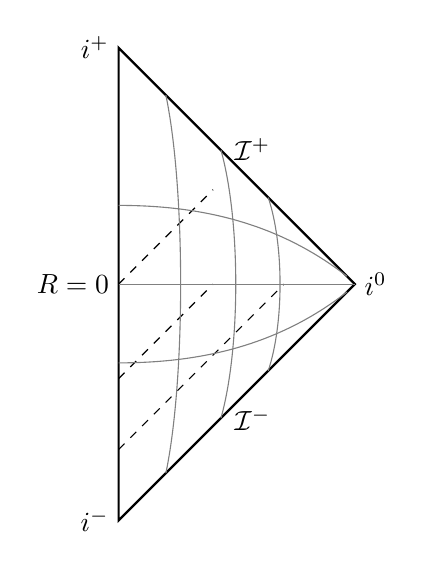
\begin{tikzpicture}[scale=1.0]
\draw[thick] (0,-3) -- (0,3) -- (3,0) -- cycle;

\node[left] at (0,3) {$i^+$};
\node[left] at (0,-3) {$i^-$};
\node[right] at (3,0) {$i^0$};
\node[left] at (0,0) {$R=0$};
\node[above right] at (1.35,1.45) {$\mathcal{I}^+$};
\node[below right] at (1.35,-1.45) {$\mathcal{I}^-$};

\draw[dashed] (0,-2.1) -- (2.1,0.0);
\draw[dashed] (0,-1.2) -- (1.2,0.0);
\draw[dashed] (0,0.0) -- (1.2,1.2);

\draw[gray] (0,0) -- (3,0);
\draw[gray] (0,1.0) .. controls (1.0,1.0) and (2.0,0.8) .. (2.9,0.1);
\draw[gray] (0,-1.0) .. controls (1.0,-1.0) and (2.0,-0.8) .. (2.9,-0.1);

\draw[gray] (0.6,-2.4) .. controls (0.85,-1.2) and (0.85,1.2) .. (0.6,2.4);
\draw[gray] (1.3,-1.7) .. controls (1.55,-0.8) and (1.55,0.8) .. (1.3,1.7);
\draw[gray] (1.9,-1.1) .. controls (2.1,-0.5) and (2.1,0.5) .. (1.9,1.1);
\end{tikzpicture}
\caption{반지름 방향으로 축약한 평탄 시공간의 페ン로즈 다이어그램. 시간 고정 곡선은 바깥쪽으로 뻗어 \(i^0\)에 이르고, 반지름 고정 곡선은 \(i^-\)에서 \(i^+\) 쪽으로 올라간다.}
\end{figure}

강의에서 마지막으로 강조한 점도 기억해야 한다. 이 다이어그램은 계량적 크기를 \emph{보존하지} 않는다. 보존하는 것은 인과 구조다. 우리가 찾는 불변량이 바로 그것이다.

\begin{classroomqa}
\audiencequestion{콤팩트화한 다이어그램에서 시간 고정 선들은 직선이어야
하나요?}
\lecturerresponse{선택한 사상에서는 대칭 단면 \(T=0\)만 직선입니다.
나머지 시간 고정 \(T\) 곡선은 휘어지며, 구체적인 모양은 콤팩트화 함수에
따라 달라집니다. 보통의 시간은 한없이 계속되지만, 매우 늦은 시간의 단면들은
위쪽 경계에 점점 더 가까이 몰립니다.
\lecturetimestamp{00:29:11--00:30:12}}
\end{classroomqa}

\section{콤팩트화한 슈바르츠실트 기하학}

평탄 공간의 구성을 바탕으로 이제 블랙홀로 돌아가 같은 작업을 한다. 영좌표를 도입하고 무한한 범위를 압축해 유한한 그림으로 만들어 크루스칼 기하학을 콤팩트화한다. 강의자는 결과를 대각선 방향의 직사각형 또는 마름모꼴 인과 그림으로 설명한다. 지평선은 영 경계로 나타나고, 바깥에서 정지해 있는 세계선은 그 바깥에 남는다. 내부 영역은 이제 페이지에 보이는 특이점에서 끝난다.

여기서 핵심적인 물리적 요점은 자유 낙하 관찰자의 경험에서 특이점이 무한히 멀리 \emph{있지 않다}는 것이다. 지평선을 넘고 나면 특이점에 부딪히기까지 남은 고유시간은 유한하다. 페ン로즈 다이어그램은 이 점을 시각적으로 분명하게 보여 준다.

지평선은 다시 슈바르츠실트 조건으로 확인된다.
\begin{equation}
1-\frac{2MG}{r}=0
\qquad \Longleftrightarrow \qquad
r=2MG.
\end{equation}
등식 \(r=2MG\)는 슈바르츠실트 인자가 부호를 바꾸는 반지름을 나타낸다.

\begin{figure}[htbp]
\centering
\includegraphics[width=0.72\textwidth]{lecture_08_figure_04.png}
\caption{형식적 확장 그림과 물리적으로 관련 있는 블랙홀 영역을 대비한 칠판 스케치. 칠판에는 빨간색으로 \emph{특이점}이라고 명시되어 있다.}
\lectureframe{00:37:59}
\end{figure}

\begin{figure}[htbp]
\centering
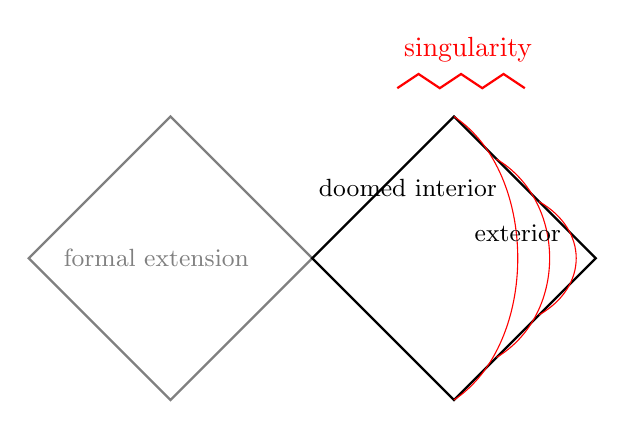
\begin{tikzpicture}[scale=0.9]
\draw[gray,thick] (-4,0) -- (-2,2) -- (0,0) -- (-2,-2) -- cycle;
\draw[thick] (0,0) -- (2,2) -- (4,0) -- (2,-2) -- cycle;

\draw[red,thick] (1.2,2.4) -- (1.5,2.6) -- (1.8,2.4) -- (2.1,2.6) -- (2.4,2.4) -- (2.7,2.6) -- (3.0,2.4);
\node[red] at (2.2,2.95) {singularity};

\draw[red] (2.0,-2.0) .. controls (3.2,-1.2) and (3.2,1.2) .. (2.0,2.0);
\draw[red] (2.6,-1.4) .. controls (3.6,-0.8) and (3.6,0.8) .. (2.6,1.4);
\draw[red] (3.2,-0.8) .. controls (3.9,-0.4) and (3.9,0.4) .. (3.2,0.8);

\node at (2.9,0.35) {\small exterior};
\node at (1.35,1.0) {\small doomed interior};
\node[gray] at (-2.2,0.0) {\small formal extension};
\end{tikzpicture}
\caption{강의에서 강조한 인과 그림을 신중하게 다시 그렸다. 남아 있는 바깥 영역, 빠져나올 수 없는 내부 영역, 미래 특이점, 그리고 확장의 추가 형식 부분과의 대비를 보여 준다.}
\end{figure}

강의의 설명은 매우 직설적이다. 바깥 영역에 있으면 탈출할 수도 있고 안으로 떨어질 수도 있다. 내부 영역에 있으면 운명을 피할 수 없다. 이 다이어그램은 미래 방향 인과 운동에 관한 중요한 내용을 이미 모두 말해 준다.

사분면 \(III\)와 \(IV\)은 최대 확장된 크루스칼 해의 정당한 부분이다. 영역 \(III\)은 두 번째 바깥 영역을 제공하고, 영역 \(IV\)는 시간 반전된 블랙홀 영역이다. 그러나 이 영역들은 붕괴로 만들어진 보통의 블랙홀 시공간에는 나타나지 않는다. 확장된 해가 수학적으로 유익한 이유는 붕괴 구성을 통해 버려야 할 부분이 무엇인지 알 수 있기 때문이다.

\section{공간 단면, 2-구, 그리고 아인슈타인--로젠 다리}

이제 콤팩트화한 다이어그램을 공간꼴 단면에서 고정해 놓고, 그 단면이 시공간이 아니라 \emph{공간}으로서는 어떤 모습인지 묻자. 여기서 웜홀 그림이 등장한다. 또한 공간적 그림이 인과 논의를 앞질러 가게 해서는 안 된다.

각도 방향을 생략했으므로 반지름 다이어그램의 각 점은 하나의 2-구를 나타낸다. 슈바르츠실트 반지름 \(r\)에서 그 면적은 다음과 같다.
\begin{equation}
A=4\pi r^2.
\end{equation}
따라서 공간꼴 단면은 단순한 1차원 곡선이 아니라 2-구들의 모임이다. 단면을 따라 이동하면 구들의 크기가 변한다.

멀리 떨어진 곳에서는 구들이 매우 크다. 안쪽으로 이동하면 구의 반지름이 줄어들다가 지평선에서 최솟값에 도달한다.
\begin{equation}
r_{\min}=2MG.
\end{equation}
형식적 확장을 지나 계속 나아가면, 구들은 다시 커져 또 다른 점근 영역으로 향한다. 이것이 아인슈타인--로젠 다리 그림이다.

\begin{figure}[htbp]
\centering
\includegraphics[width=0.72\textwidth]{lecture_08_figure_05.png}
\caption{다리 기하학을 구성하는 데 사용한 초록색 공간꼴 단면을 포함한 확장 크루스칼 다이어그램. 이 단면의 모든 점은 2-구 하나를 나타내며, 최소 반지름 위치는 \(r=2MG\)로 표시되어 있다.}
\lectureframe{00:41:30}
\end{figure}

칠판에는 슈바르츠실트 인자의 일부만 표시되어 있다.
\begin{equation}
1-\frac{2MG}{r},
\end{equation}
목 부분은 같은 특별한 반지름 \(r=2MG\)에 위치한다.

\begin{figure}[htbp]
\centering
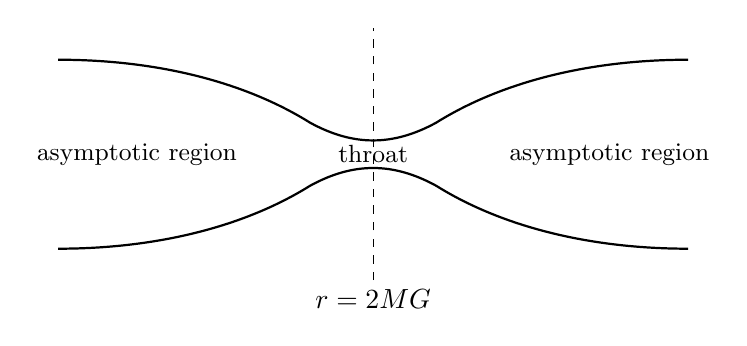
\begin{tikzpicture}[scale=1.0]
\draw[thick] (-4,1.2)
.. controls (-2.7,1.2) and (-1.6,0.9) .. (-0.8,0.4)
.. controls (-0.25,0.1) and (0.25,0.1) .. (0.8,0.4)
.. controls (1.6,0.9) and (2.7,1.2) .. (4,1.2);

\draw[thick] (-4,-1.2)
.. controls (-2.7,-1.2) and (-1.6,-0.9) .. (-0.8,-0.4)
.. controls (-0.25,-0.1) and (0.25,-0.1) .. (0.8,-0.4)
.. controls (1.6,-0.9) and (2.7,-1.2) .. (4,-1.2);

\draw[dashed] (0,-1.6) -- (0,1.6);
\node[below] at (0,-1.6) {$r=2MG$};
\node at (0,0) {\small throat};
\node at (-3.0,0) {\small asymptotic region};
\node at (3.0,0) {\small asymptotic region};
\end{tikzpicture}
\caption{확장 슈바르츠실트 기하학을 가로지르는 공간 단면의 개략도. 이것은 강의의 다리 그림을 신중하게 재구성한 것이며, 실제 매장 계산을 나타내지는 않는다.}
\end{figure}

이제 수정할 점이 나온다. 단면은 두 점근 영역 사이의 다리를 보여 주므로, 목을 지나 한 우주에서 다른 우주로 이동할 수 있지 않을까 하는 생각을 불러일으킨다. 강의에서는 먼저 그런 생각이 떠오르게 한 뒤, 인과 구조를 따져 이를 부정한다. 한 바깥 영역에서 다른 바깥 영역으로 가려면 페ン로즈 다이어그램 어딘가에서 세계선이 \(45^\circ\) 영선보다 완만해져야 한다. 이는 허용되지 않는다. 그러므로 아인슈타인--로젠 다리는 통과할 수 없다.

강의자는 공간적 그림이 오해를 부를 수 있는 이유도 강조한다. 이것은 한순간의 \emph{공간}을 그린 그림일 뿐이지만, 통과할 인과적 시간은 충분하지 않다. 느슨하게 말하면, 무엇이든 건너가기 전에 다리가 열렸다 닫힌다고 할 수 있다. 더 나은 방법은 페ン로즈 다이어그램을 다시 보고 인과적 답을 읽는 것이다.

\section{유입하는 영 껍질로 실제 블랙홀 만들기}

이 지점에서 강의의 문제가 완전히 바뀐다. 더는 영원한 블랙홀의 성질을 읽어 내지 않는다. 실제 블랙홀을 구성한다.

단순성을 위해 모형을 택한다. 내부 구조가 복잡한 붕괴 별이 아니라, 얇은 구형 유입 복사 껍질을 상상한다. 이것은 빛의 껍질이므로 빛의 속도로 안쪽을 향해 움직인다. 충분히 작은 반지름에 이르면 껍질에 실린 에너지가 블랙홀을 형성할 만큼 좁은 영역에 집중된다.

두 번째 요소는 일반상대론에서의 껍질 정리다.

\paragraph{비고.} 이 강의에서 다루는 구대칭 껍질에서는 내부 영역이 평탄 시공간이고 외부 영역은 슈바르츠실트 시공간이다. 이것이 강의에서 사용하는 실질적인 껍질 정리, 즉 버코프 정리 유형의 진술이다. 여기서 이를 증명하지는 않는다.

강의자는 먼저 뉴턴 역학의 껍질 정리를 되짚어 이를 설명한다. 구형 껍질 안에는 중력장이 없고, 껍질 바깥의 중력장은 중심에 있는 점질량의 장과 같다. 이어서 여기서 필요한 형태로 대응하는 상대론적 진술을 제시한다. 안쪽은 평탄하고 바깥쪽은 슈바르츠실트 시공간이다. 껍질이 움직여도 이 규칙은 같다.

이것으로 붕괴 시공간을 구성하기에 충분하다. 껍질 자체가 영이므로 \(45^\circ\)로 그려야 한다. 이 영선의 한쪽은 평탄한 기하학이고 다른 쪽은 슈바르츠실트 기하학이다. 다음과 같이 규칙을 요약할 수 있다.
\begin{equation}
\begin{aligned}
\text{inside shell} &= \text{flat spacetime},\\
\text{outside shell} &= \text{Schwarzschild geometry}.
\end{aligned}
\end{equation}

그러면 이어 붙이는 방법은 놀라울 만큼 간단해진다.

\begin{enumerate}
\item 평탄 시공간의 페ン로즈 다이어그램을 그리고 유입 껍질 안쪽 영역만 남긴다.
\item 슈바르츠실트 페ン로즈 다이어그램을 그리고 같은 껍질 바깥쪽 영역만 남긴다.
\item 잘못된 부분들을 버린다.
\item 남은 두 부분을 껍질의 궤적을 따라 이어 붙인다.
\end{enumerate}

강의는 바로 이 순서대로 칠판에서 진행된다. 한 그림의 잘못된 절반을 버리고, 다른 그림의 잘못된 절반도 버린 다음, 올바른 절반끼리 껍질을 따라 이어 붙인다.

\begin{figure}[htbp]
\centering
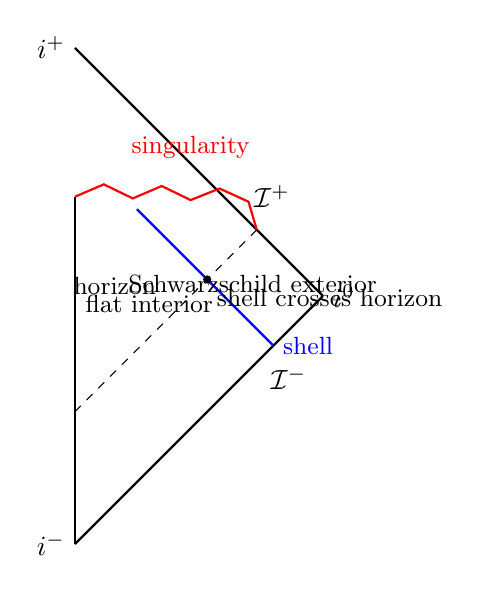
\begin{tikzpicture}[scale=1.05]
\coordinate (im) at (0,-3.0);
\coordinate (ip) at (0,3.0);
\coordinate (i0) at (3.0,0.0);
\coordinate (S)  at (0,1.2);
\coordinate (E)  at (2.2,0.8);
\coordinate (P)  at (2.4,-0.6);
\coordinate (Q)  at (0.75,1.05);
\coordinate (H)  at (0,-1.4);
\coordinate (X)  at (1.6,0.2);

\draw[thick] (im) -- (S);
\draw[thick] (im) -- (i0);
\draw[thick] (ip) -- (i0);

\draw[red,thick] (S) -- (0.35,1.35) -- (0.7,1.18) -- (1.05,1.33) -- (1.4,1.16) -- (1.75,1.30) -- (2.1,1.14) -- (E);
\node[red,above] at (1.4,1.55) {\small singularity};

\draw[thick,blue] (P) -- (Q);
\node[blue,right] at (P) {\small shell};

\draw[dashed] (H) -- (E);
\node[above left] at (1.1,-0.1) {\small horizon};

\filldraw (X) circle (1.2pt);
\node[below right] at (X) {\small shell crosses horizon};

\node at (0.9,-0.1) {\small flat interior};
\node at (2.15,0.15) {\small Schwarzschild exterior};

\node[left] at (im) {$i^-$};
\node[left] at (ip) {$i^+$};
\node[right] at (i0) {$i^0$};
\node[below right] at (2.25,-0.75) {$\mathcal{I}^-$};
\node[above right] at (2.05,0.95) {$\mathcal{I}^+$};
\end{tikzpicture}
\caption{붕괴 기하학의 인과 구조를 재구성한 그림. 껍질은 안쪽으로 향하는 영선이며, 그 안쪽에는 평탄 시공간을, 바깥쪽에는 슈바르츠실트 기하학을 남긴다.}
\end{figure}

\begin{figure}[htbp]
\centering
\includegraphics[width=0.76\textwidth]{lecture_08_figure_06.png}
\caption{평탄한 내부와 슈바르츠실트 외부를 유입하는 파란 껍질을 따라 이어 붙인 뒤의 칠판 구성. 점선 \(45^\circ\)은 미래 특이점의 끝점에서 거꾸로 추적해 사건의 지평선을 찾고 있다.}
\lectureframe{00:57:30}
\end{figure}

껍질은 다이어그램의 평탄한 부분에서 슈바르츠실트 부분으로 넘어갈 때 특별한 일을 겪지 않는다. 빛꼴 껍질은 안쪽으로 계속 이동해 특이점에 이른다. 핵심 구조는 껍질 위에서 벌어지는 국소적인 사건이 아니라, 이어 붙인 시공간의 인과적 배치에 담겨 있다.

\begin{classroomqa}
\audiencequestion{붕괴하는 껍질이 슈바르츠실트 반지름을 지날 때 불연속이
생기나요?}
\lecturerresponse{아닙니다. 그 지점에서 국소적으로 특이한 일은 일어나지
않습니다. 껍질은 영궤적을 따라 계속 움직입니다. 인과적으로 특별한 사건은
껍질이 자신의 \(2MG\) 반지름을 지난 뒤에는 미래 방향의 어떤 경로도 무한대까지
되돌아갈 수 없다는 것입니다.
\lecturetimestamp{00:56:19--00:56:42}}
\end{classroomqa}

\section{도착하기 전의 지평선: 사건의 지평선 문제}

이제 강의의 개념적 절정에 이르렀다. 붕괴 시공간을 구성하고 나면 자연스러운 질문이 생긴다. 지평선은 어디에 있는가? 강의자의 표현을 빌리면, 돌아올 수 없는 지점은 어디인가?

\paragraph{정의.} 사건의 지평선은 미래 방향의 인과 신호를 \(\mathcal{I}^+\)에 보낼 수 있는 사건들과 보낼 수 없는 사건들을 가르는 경계다.

강의에서는 다이어그램을 이용해 사건의 지평선을 찾는다. 특이점이 미래 영무한대와 만나는 꼭짓점에서 시작해 \(45^\circ\) 영선을 거꾸로 추적한다. 그렇게 거꾸로 추적한 영선이 사건의 지평선이다.

그러나 강의자는 학생들을 불편하게 하는 두 번째 요점을 강조한다. 지평선은 껍질이 자신의 슈바르츠실트 반지름을 지나는 순간에 나타나서 그대로 머무는 것이 아니다. 칠판을 확장해 그리면 지평선은 중심 근처의 아주 작은 포획 영역에서 시작해 아직 평탄한 시공간의 일부를 지나 바깥쪽으로 자라며, 한참 뒤에 유입 껍질과 만난다. 그 만남의 순간에 껍질은 자신의 슈바르츠실트 반지름을 지난다. 그 순간보다 위쪽에서는 완성된 블랙홀의 보통의 반지름 고정 지평선이 된다.

\begin{figure}[htbp]
\centering
\resizebox{0.96\linewidth}{!}{%
\begin{tikzpicture}[scale=1.08,>=Latex]
\coordinate (im) at (0,-3.0);
\coordinate (ip) at (0,3.0);
\coordinate (i0) at (3.0,0.0);
\coordinate (S)  at (0,1.2);
\coordinate (E)  at (2.2,0.8);
\coordinate (P)  at (2.4,-0.6);
\coordinate (Q)  at (0.75,1.05);
\coordinate (H)  at (0,-1.4);
\coordinate (X)  at (1.6,0.2);

\draw[thick] (im) -- (S);
\draw[thick] (im) -- (i0);
\draw[thick] (ip) -- (i0);

\draw[red,thick] (S) -- (0.35,1.35) -- (0.7,1.18) -- (1.05,1.33) -- (1.4,1.16) -- (1.75,1.30) -- (2.1,1.14) -- (E);
\node[red,above left] at (S) {\small singularity};

\draw[very thick,red] (H) -- (E);

\draw[thick,blue] (P) -- (Q);

\filldraw (X) circle (1.2pt);

\draw[gray] (0.0,-2.1) .. controls (0.85,-1.95) and (1.9,-1.3) .. (2.8,-0.2);
\draw[gray] (0.0,-1.2) .. controls (0.95,-1.0) and (1.8,-0.45) .. (2.45,0.35);
\draw[gray] (0.0,-0.2) .. controls (0.8,-0.05) and (1.45,0.35) .. (1.95,0.95);

\node[below right] at (2.28,-0.72) {$\mathcal{I}^-$};
\node[above right] at (2.12,0.92) {$\mathcal{I}^+$};

\draw[very thick,red] (3.2,-1.15) -- (3.75,-1.15);
\node[anchor=west] at (3.85,-1.15) {\small event horizon};
\draw[thick,blue] (3.2,-1.55) -- (3.75,-1.55);
\node[anchor=west] at (3.85,-1.55) {\small infalling shell};
\filldraw (3.48,-1.95) circle (1.2pt);
\node[anchor=west] at (3.85,-1.95)
  {\small shell reaches \(r=2MG\)};
\end{tikzpicture}
}
\caption{거꾸로 추적한 사건의 지평선을 강조한 붕괴 다이어그램. 지평선의 일부는 여전히 국소적으로 평탄하고 껍질이 아직 도달하지 않은 영역에 놓인다.}
\end{figure}

이것이 강의의 나머지 부분에서 거듭 다루는 놀라운 효과다. 지평선의 일부는 평탄한 시공간에 놓인다. 껍질은 아직 그곳에 도착하지 않았고, 관찰자의 과거 광원뿔에도 보이지 않는다. 관찰자는 중력장을 느끼지 않는데도 탈출할 수 없다. 그 이유는 국소적인 힘이 아니라 사건의 전역적 인과적 미래에 있다.

\begin{classroomqa}
\audiencequestion{이 구성은 껍질을 건널 수 없다는 뜻인가요, 아니면 지평선을
건널 수 없다는 뜻인가요? 지평선이 껍질 안쪽에 있을 때 껍질은 어디에 있나요?}
\lecturerresponse{껍질은 건널 수 있습니다. 지평선은 별개의 영곡면으로,
서로 \(\mathcal I^+\)와 인과적으로 소통할 수 있는 사건들과 그럴 수 없는 사건들을 가르는
경계입니다. 유입 껍질은 전체 에너지에 해당하는 슈바르츠실트 반지름을 지날 때
정확히 그 경계와 만납니다. 만나기 전에는 사건의 지평선 일부가 평탄한 내부를
지나며, 만난 뒤에는 껍질이 완성된 블랙홀 안에 놓입니다.
\lecturetimestamp{00:58:42--01:01:06}}
\end{classroomqa}

\begin{classroomqa}
\audiencequestion{내부가 평탄하고 껍질이 아직 멀리 떨어져 있다면, 지평선 바로 안쪽에 있는 사람은 껍질이 도착하기 전에 왜 그곳을 걸어서 빠져나올 수 없을까요?}
\lecturerresponse{바깥쪽으로 향하는 가장 빠른 세계선을 그려 봅시다. 그것은 \(45^\circ\)빛의 광선입니다. 과거 방향으로 추적한 지평선 안쪽의 사건에서 출발한 광선조차 유입하는 껍질과 너무 늦게 만나 특이점에 도달합니다. 걷는 속도는 그보다도 느립니다. \emph{껍질이 아직 통과하지 않았다}라는 말은 시간 좌표를 정하기 전까지는 불완전합니다. 인과 도표가 좌표계와 무관한 답을 줍니다. 유입하는 우주 마이크로파 배경 복사는 같은 사례가 아닙니다. 이 기하를 만들어 내는 것은 붕괴하는 구형 껍질이 아니기 때문입니다.
\lecturetimestamp{01:01:07--01:04:03}}
\end{classroomqa}

\section{거울과 미래를 바꾸려는 시도}

이제 질문들은 다이어그램을 실험실로 바꾼다. 유입하는 빛 껍질이 포획되기 전에 반사될 수 있다고 가정해 보자. 그러면 가정한 붕괴 이력이 바뀌고 사건의 지평선도 달라진다. 모순은 아니다. 사건의 지평선은 완전한 시공간의 역사가 정해진 뒤에야 정의되기 때문이다.

\begin{classroomqa}완벽한 반사 거울을 블랙홀이 생길 것으로 예상되는 슈바르츠실트
반지름 바로 바깥에 놓아 껍질이 되돌아 나오게 하면 어떻게 되나요?\audiencequestion{
}이 이상화된 이력에서는 유입 영선이 거울에서 바깥쪽으로 꺾여
미래 경계에 도달합니다. 원래 다이어그램의 블랙홀은 형성되지 않습니다.
무게가 전혀 없는 거울은 불가능하고 실제 거울은 자체 응력 에너지도 더하지만,
이 사고실험은 논리적 요점을 분명히 합니다. 껍질이 실제 사건의 지평선을 지난
뒤에야 탈출이 불가능해집니다.
\lecturerresponse{
\lecturetimestamp{01:04:33--01:05:54}}
\end{classroomqa}

\begin{classroomqa}껍질이 온다는 사실을 미리 안 관찰자가 거울이나 신호를
재빨리 보내 껍질을 되돌릴 수 있나요?\audiencequestion{
}필요한 장치를 지평선 바깥에 충분히 일찍 설치할 수 있을 때만
가능합니다. 앨리스는 밥에게 껍질을 보내도록 미리 부탁할 수 있으므로, 껍질을
보기 전에 무엇이 올지 알 수도 있습니다. 그러나 앨리스가 있는 사건이 지평선
안쪽에 놓인 뒤에는 거울도 지시도 제때 필요한 바깥 지점에 도달할 수 없습니다.
미래의 실험을 안다고 해서 다이어그램이 금지하는 인과 경로가 열리지는 않습니다.
\lecturerresponse{
\lecturetimestamp{01:05:55--01:08:18}}
\end{classroomqa}

\begin{classroomqa}이미 지평선 안에 있는 거울은 어떻게 되나요? 특이점은 그 거울의
미래에서 무한히 멀리 있나요?\audiencequestion{
}거울도 운명을 피할 수 없는 또 하나의 물체일 뿐입니다. 국소적으로
빛을 반사할 수는 있지만, 반사된 빛과 거울, 앨리스는 모두 특이점에서 끝납니다.
일반적인 자유 낙하 세계선은 유한한 고유시간 안에 특이점에 도달합니다.
콤팩트화 다이어그램의 이상적인 위쪽 꼭짓점만 무한히 멀리 있습니다. 그 꼭짓점
근처에 머물려면 한계 없이 커지는 가속도와 에너지가 필요합니다. 게다가 고정된
두 사건 사이에서 가속하는 시계가 누적하는 고유시간은 관성 시계보다 더 긴 것이
아니라 짧습니다.
\lecturerresponse{
\lecturetimestamp{01:08:19--01:10:19}}
\end{classroomqa}

\begin{classroomqa}붕괴하는 껍질이 거대하다면, 껍질 안쪽에 있으면서 최종 중심에서
멀리 떨어진 사람은 껍질이 지나가는 동안 그 자리에 그대로 있을 수 있나요?\audiencequestion{
}네. 그 사람이 있는 사건이 여전히 사건의 지평선 바깥이라면
가능합니다. 물질 껍질 안쪽에 있다는 것과 블랙홀 안쪽에 있다는 것은 같은 말이
아닙니다. 복사가 관찰자에게 부딪혀 상처를 입힐 수는 있지만, 그것은 껍질과의
국소적 상호작용이며 탈출 가능성이라는 인과적 문제와는 별개입니다.
\lecturerresponse{
\lecturetimestamp{01:10:21--01:11:24}}
\end{classroomqa}

\section{시간 단면과 성장하는 지평선}

곡률이 있는 시공간에서 \emph{시간의 한 순간}이란 선택된 공간꼴 초곡면을 뜻합니다. 이런 초곡면을 쌓아 놓은 것이 엽층화이며, 각 초곡면에 하나의 수를 대응시키면 시간 좌표가 정의됩니다. 서로 다른 엽층화는 동일한 붕괴 도표를 서로 다르게 가릅니다. 어느 먼 사건들이 동시인지에 대해서는 서로 다른 답을 내지만, 어떤 영선이 무한대에 도달하는지는 바꾸지 않습니다.

\begin{figure}[htbp]
\centering
\includegraphics[width=0.77\textwidth]{lecture_08_figure_07.png}
\caption{뒤쪽 칠판에 그려진 여러 개의 초록색 공간꼴 단면 도표. 이 단면들은 시간 좌표를 정의하며, 검은색 영 경계와 그 인과 관계는 그 선택과 무관하다.}
\lectureframe{01:17:30}
\end{figure}

\begin{classroomqa}
\audiencequestion{한순간에 관측자와 지평선 사이의 거리와 지평선과 껍질 사이의 거리를 비교하는 방식으로 이 문제를 다시 말할 수 있을까요?}
\lecturerresponse{엽층화를 정한 뒤에는 유용한 직관을 얻는 방법이 될 수 있지만, \emph{한순간에}라는 표현은 좌표계에 따라 달라집니다. 명확하게 구성하려면 공간꼴 단면들의 모음을 그리면 됩니다. 이른 단면은 큰 껍질과 만나며, 갇힌 중앙 영역과는 만나지 않습니다. 더 늦은 단면은 여전히 안쪽으로 낙하하는 껍질 안쪽에서 커지고 있는 지평선과 만납니다. 하나의 특별한 단면은 껍질이 자신의 슈바르츠실트 반지름을 통과하는 사건을 지납니다.
\lecturetimestamp{01:11:26--01:14:21}}
\end{classroomqa}

\begin{classroomqa}
\audiencequestion{지평선이 바깥쪽으로 열리면서 슈바르츠실트 반지름도 커지나요? 껍질이 지평선을 통과한 뒤에도 지평선이 계속 커지는 이유는 무엇인가요?}
\lecturerresponse{최종 슈바르츠실트 반지름 \(2MG\)은 전체 질량 \(M\)이 고정되어 있으므로 고정되어 있습니다. 이른 공간꼴 단면에서 커지는 것은 지평선 단면의 면적 반지름입니다. 중심에서 시작해 \(r=2MG\)에서 껍질과 만날 때까지 증가한 뒤 멈춥니다. 그 만남 사건 위쪽에서 지평선은 \(r\)이 일정한 \(r=2MG\) 선입니다. 다만 압축한다고 해서 그 선이 수직이 되거나 계량상 균일해지는 것은 아닙니다.
\lecturetimestamp{01:14:22--01:16:15}}
\end{classroomqa}

\begin{classroomqa}
\audiencequestion{처음에 최종 슈바르츠실트 반지름의 절반 지점에 있던 관측자는 어떻게 되나요? 껍질이 도착해야 비로소 중력을 느끼는 것 아닌가요?}
\lecturerresponse{그렇습니다. 관측자는 시공간이 여전히 평탄할 때 먼저 커지고 있는 사건지평선을 통과하며, 갑작스러운 힘을 느끼지 않습니다. 안쪽으로 낙하하는 복사 껍질은 물질이므로 나중에 감지될 수 있지만, 사건지평선은 그렇지 않습니다. 지평선을 통과한다는 것은 이제 미래 방향의 모든 인과 경로가 무한대에 도달하지 못한다는 뜻일 뿐입니다. 이런 엄밀한 의미에서 지평선은 유령과 같습니다.
\lecturetimestamp{01:16:17--01:17:45}}
\end{classroomqa}

\begin{classroomqa}
\audiencequestion{충분히 일찍 출발한 관측자는 커지는 지평선보다 더 빠르게 바깥쪽으로 움직여 탈출할 수 있나요?}
\lecturerresponse{지평선 바깥의 사건에는 \(\mathcal I^+\)에 도달하는 바깥쪽 인과 경로가 있지만, 안쪽의 사건에는 그런 경로가 없습니다. 선택한 단면 위에서 쓸 수 있는 반지름 방향 거리와 유입하는 껍질이 경로를 닫기까지의 시간을 비교할 수는 있지만, 정확한 판정 기준은 영선입니다. 관측자에게 물질로 된 지평선이 바깥쪽으로 돌진하는 모습이 보이지는 않습니다. 국소적으로 볼 수 있는 표면은 없기 때문입니다.
\lecturetimestamp{01:17:46--01:18:54}}
\end{classroomqa}

\section{도표가 보존하는 것}

페이지에 그려진 모양을 축척도처럼 읽어서는 안 됩니다. 작은 모퉁이가 시공간의 무한한 영역을 나타낼 수도 있고, 넓은 부분이 물리적으로는 얼마 되지 않는 구간을 나타낼 수도 있습니다. 압축은 영 방향을 보존하기 위해 의도적으로 계량적 크기를 희생합니다. 보존되는 것은 인과관계입니다. 누가 누구에게 신호를 보낼 수 있는지, 어떤 사건이 다른 어떤 사건에 영향을 줄 수 있는지, 그리고 어떤 세계선이 빛의 속도 제한으로 인해 갇히는지가 남습니다.

\begin{classroomqa}
\audiencequestion{그림이 길이와 시간을 이토록 심하게 왜곡한다면, 무엇을 충실하게 나타내나요?}
\lecturerresponse{빛의 광선, 따라서 인과 구조를 나타냅니다. 사건지평선을 찾으려면 미래 무한대에서 마지막 바깥쪽 영선을 거슬러 추적하면 됩니다. 페이지에 보이는 거리만으로 답을 추론하는 것은 신뢰하기 어렵습니다. 인과 도표를 그려 두면 계량의 축척이 생략되어 있어도 신호, 탈출, 그리고 돌아올 수 없음에 관한 질문에 기하학적인 답을 얻을 수 있습니다.
\lecturetimestamp{01:18:56--01:21:45}}
\end{classroomqa}

\begin{classroomqa}
\audiencequestion{펜로즈 도표를 직관적으로 사용할 만큼 익숙해지는 데 얼마나 걸리나요?}
\lecturerresponse{오래 걸리지 않습니다. 실제로는 도표를 그리고, 영선을 추적하고, 가능한 세계선들을 검토하다 보면 인과적 제약에 익숙해집니다. 여기서 직관은 도표 없이 짐작해서 얻는 것이 아니라 도표를 다루면서 익히는 것입니다.
\lecturetimestamp{01:21:49--01:22:05}}
\end{classroomqa}

\begin{classroomqa}
\audiencequestion{이런 시각적 방법은 수학이 그림보다 더 믿을 만한 경우가 많은 양자역학과 정반대인가요?}
\lecturerresponse{상당한 정도로 그렇습니다. 일반상대성이론은 고전물리학입니다. 휘어진 4차원 시공간을 문자 그대로 머릿속에 그리기는 어렵고 펜로즈 도표도 여전히 추상적이지만, 그 인과 기하는 양자역학의 근본적인 실재보다 훨씬 더 많이 그려 보고 탐구할 수 있습니다. 이런 차이가 이 도표를 매우 강력하게 만드는 이유 중 하나입니다.
\lecturetimestamp{01:22:05--01:22:58}}
\end{classroomqa}